\documentclass[pdf]{beamer}
\mode<presentation>{} 

\usepackage{hyperref}
\usepackage{pgf}
\usepackage{tikz}
\usepackage{multicol}
\usepackage{graphicx}
\usepackage{eso-pic}
\usetikzlibrary{patterns}
\usetikzlibrary{trees}
\usetikzlibrary{arrows,automata}
\usetikzlibrary{automata,positioning}
\usetikzlibrary{shapes}
\usepackage{tikz-qtree,tikz-qtree-compat}
\usepackage{mathtools,enumerate,amssymb}
\usepackage[utf8]{inputenc}
\usepackage[T1]{fontenc}
\usepackage{graphicx}
\usepgflibrary{arrows}
\usepackage{multirow}
\usepackage[export]{adjustbox}
\usepackage{wrapfig}




\definecolor{Blue}{RGB}{0,0,100}
\definecolor{background}{RGB}{255,255,255}



\newcommand\tab[1][1cm]{\hspace*{#1}}
\newcommand{\dialogueline}[2]{\begin{dialogue}{#1} #2 \end{dialogue}}



\title{Pathological designs}
\subtitle{Human Computer Interaction}
\AtBeginSection[]{}



\setbeamertemplate{sidebar right}{}
\setbeamertemplate{footline}{%
\hfill\usebeamertemplate***{navigation symbols}
\hspace{1cm}\insertframenumber{}/\inserttotalframenumber}

\graphicspath{{./img/}}



\begin{document}



{\setbeamercolor{background canvas}{bg=background}
\begin{frame}
\vspace{10mm}
\huge{\raggedleft{\color{black}{\textbf{Pathological Designs}}}}

\large{\raggedleft{\color{black} Human Computer Interaction}}

\begin{flushright}
\end{flushright}

\fontsize{7pt}{1pt}\selectfont{
Based on slide deck 

\textbf{Part 4: Designing and building visual interfaces. Pathological Designs}

Human Computer Interaction I: Principles and Design

by

\textbf{Saul Greenberg}
\newline
Professor
\newline
\textbf{University of Calgary, Canada}

\textit{The new slides are marked with a *}
}

\fontsize{5pt}{1pt}\selectfont{ \textcolor{lightgray}
{Slide deck by Saul Greenberg. Permission is granted to use this for non-commercial purposes as long as general credit to Saul Greenberg is clearly maintained.
Warning: some material in this deck is used from other sources without permission. Credit to the original source is given if it is known.}}

\end{frame}}



%--------------------------------------
% Iuga Alexandru
% 1
{
\setbeamertemplate{footline}[text line]{ \noindent\parbox{\linewidth}{\hfill \hspace*{-30pt}{ \vfill \vspace*{-25pt}{ \tiny{ \textcolor{gray}{Slide deck by Saul Greenberg. Permission is granted to use this for non-commercial purposes as long as general credit to Saul Greenberg is clearly maintained. Notice: some material in this deck is used from other sources without permission. Credit to the original source is given if it is known.}}}} }}
\begin{frame}
\begin{center}{ \huge{\textbf {\usebeamercolor[fg]{title}{Design of Everyday Things }}}}
\end{center}

\begin{itemize}
\item[] Pathological designs
\item[] Many human errors result from design errors
\item[] Designers help through a good conceptual model
\end{itemize}
\end{frame}}



%--------------------------------------
% Iuga Alexandru
% 2
% 2_cezar.jpg
% 2_cloudToRight.png
\begin{frame}
    \textcolor{Blue}{\textbf{\Large{41 BC: Emperor tired of loosing to the Gauls}}}
    \textcolor{red}{\rule{10cm}{1mm}}

\begin{figure}[h] \begin{flushleft}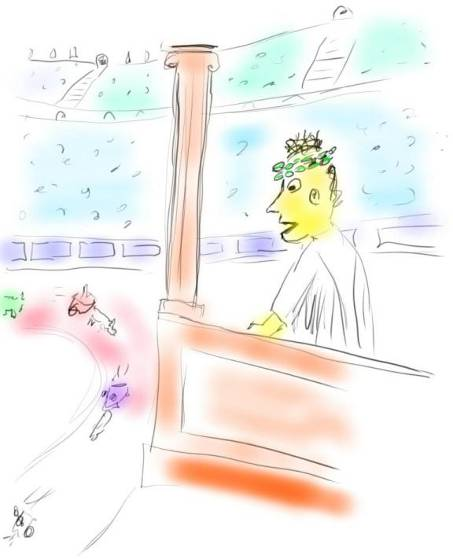
\includegraphics[height=7.3cm]{2_cezar.jpg}
\end{flushleft} \end{figure}
\leavevmode\makebox(0,0){\put(130,370){
\includegraphics[height=2cm]{2_cloudToRight.png}}}
\leavevmode\makebox(0,0){\put(138,398){\fontfamily{comic}{\selectfont{\bf{ Win me the}}}}}
\leavevmode\makebox(0,0){\put(138,375){\fontfamily{comic}\selectfont\bf{Chariot Race } }}
%footer
\leavevmode\makebox(0,0){\put(-20,40){\tiny{\textcolor{gray}{Slide idea from David Hill}}}}
\leavevmode\makebox(0,0){\put(270,40){\tiny{\textcolor{gray}{Saul Greenberg}}}}
\end{frame}



%--------------------------------------
% Iuga Alexandru
% 3
% 3_witch.png
% 3_cloudToLeft.png
\begin{frame}
    \textcolor{Blue}{\textbf{\Large{Advisor intuitively finds a solution ...}}}
    \textcolor{red}{\rule{10cm}{1mm}}

\begin{figure}[h] \begin{flushright}
	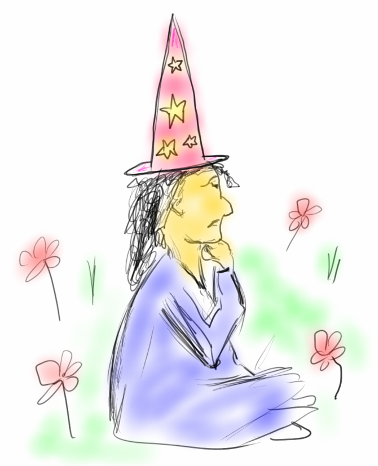
\includegraphics[width=0.55\textwidth]{3_witch.png}
\end{flushright} \end{figure}
\leavevmode\makebox(0,0){\put(110,375){
\includegraphics[height=3.35cm]{3_cloudToLeft.png}}}
\leavevmode\makebox(0,0){\put(120,430){\fontfamily{comic}{\selectfont{\bf{ Hmm......}}}}}
\leavevmode\makebox(0,0){\put(123,384){\fontfamily{comic}{\selectfont{\bf{ AHA!}}}}}
\leavevmode\makebox(0,0){\put(108,360){\fontfamily{comic}{\selectfont{\bf{The Wind!}}}}}
%footer
\leavevmode\makebox(0,0){\put(-20,40){\tiny{\textcolor{gray}{Slide idea from David Hill}}}}
\leavevmode\makebox(0,0){\put(270,40){\tiny{\textcolor{gray}{Saul Greenberg}}}}
\end{frame}



%--------------------------------------
% Iuga Alexandru
% 4
% 4_race.png
% 4_cloudToLeft.png
% 4_cloudToRight.png
\begin{frame}
    \textcolor{Blue}{\textbf{\Large{The Chariot Race}}}
    \textcolor{red}{\rule{10cm}{1mm}}

\vspace{5mm}

\leavevmode\put(-15,3){\fontfamily{comic} \fontsize{15}{11}\selectfont{\bf{ Notice aerodynamic efficiency of the faster }}}
\leavevmode\makebox(0,0){\put(-15,-30){\fontfamily{comic} \fontsize{15}{11}\selectfont{ \bf{chariot}}}}
\newline

\begin{figure}[h] \begin{flushright}
	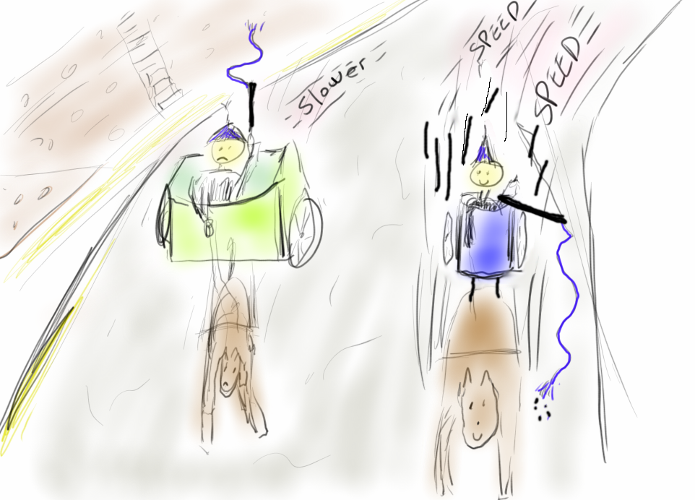
\includegraphics[width=0.885\textwidth]{4_race.png}
\end{flushright} \end{figure}
\leavevmode\makebox(0,0){\put(232,400){
\includegraphics[height=2.15cm]{4_cloudToRight.png}}}
\leavevmode\makebox(0,0){\put(246,438){\fontfamily{comic}{\selectfont{\bf{Yes!!!}}}}}
\leavevmode\makebox(0,0){\put(55,360){
\includegraphics[height=1.25cm]{4_cloudToLeft.png}}}
\leavevmode\makebox(0,0){\put(63,373){\fontfamily{comic}{\selectfont{\bf{ Nuts...}}}}}
%footer
\leavevmode\makebox(0,0){\put(-20,40){\tiny{\textcolor{gray}{Slide idea from David Hill}}}}
\end{frame}



%--------------------------------------
% Iuga Alexandru
% 5
% 5_racing.png
% 5_cloudToLeft.png
% 5_cloudToLeftBigger.png
\begin{frame}
    \textcolor{Blue}{\textbf{\Large{The Chariot Race}}}
    \textcolor{red}{\rule{10cm}{1mm}}

\vspace{5mm}

\leavevmode\put(-15,3){\fontfamily{comic} \fontsize{13}{11}\selectfont{\bf{ But, in maneuvering for position on the turn,}}}
\leavevmode\makebox(0,0){\put(-15,-30){\fontfamily{comic} \fontsize{13}{11}\selectfont{ \bf{the DRIVER makes an error!}}}}
\begin{figure}[h] \begin{flushright}
	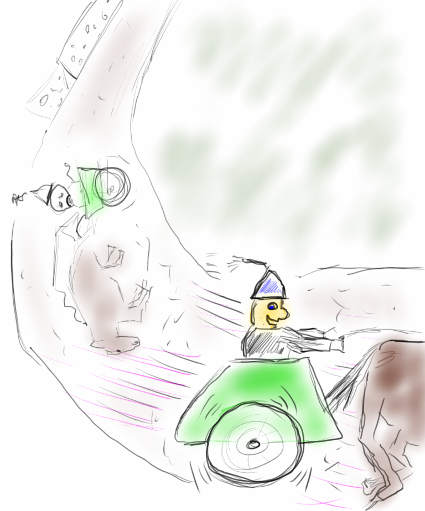
\includegraphics[scale=0.48]{5_racing.png}
\end{flushright} \end{figure}
\leavevmode\makebox(0,0){\put(210,290){
\includegraphics[height=2cm]{5_cloudToLeftBigger.png}}}
\leavevmode\makebox(0,0){\put(215,320){\fontfamily{comic}{\selectfont{\bf{\scriptsize {Har,}}}}}}
\leavevmode\makebox(0,0){\put(212,300){\fontfamily{comic}{\selectfont{\bf{\scriptsize {har...}}}}}}
\leavevmode\makebox(0,0){\put(104,310){
\includegraphics[height=1cm]{5_cloudToLeft.png}}}
\leavevmode\makebox(0,0){\put(110,327){\fontfamily{comic}{\selectfont{\bf{\scriptsize Ooops}}}}}

\leavevmode\makebox(0,0){\put(-15,120){\fontfamily{comic} \fontsize{13}{11}\selectfont{ \bf{Or was it the DESIGNER???}}}}

%footer
\leavevmode\makebox(0,0){\put(-20,75){\tiny{\textcolor{gray}{Slide idea from David Hill}}}}
\leavevmode\makebox(0,0){\put(255,75){\tiny{\textcolor{gray}{Saul Greenberg}}}}
\end{frame}



%--------------------------------------
% Iuga Alexandru
% 6
% 6_chemestryWitch.png
% 6_cloudToTheLeft.png
\begin{frame}
    \textcolor{Blue}{\textbf{\Large{Human factors engineered}}}
    \textcolor{red}{\rule{10cm}{1mm}}

\vspace{5mm}

\leavevmode\put(-15,3){\fontfamily{comic} \fontsize{13}{11}\selectfont{ \bf{- Boadiceaised as well}}}
\begin{figure}[h] \begin{center}
	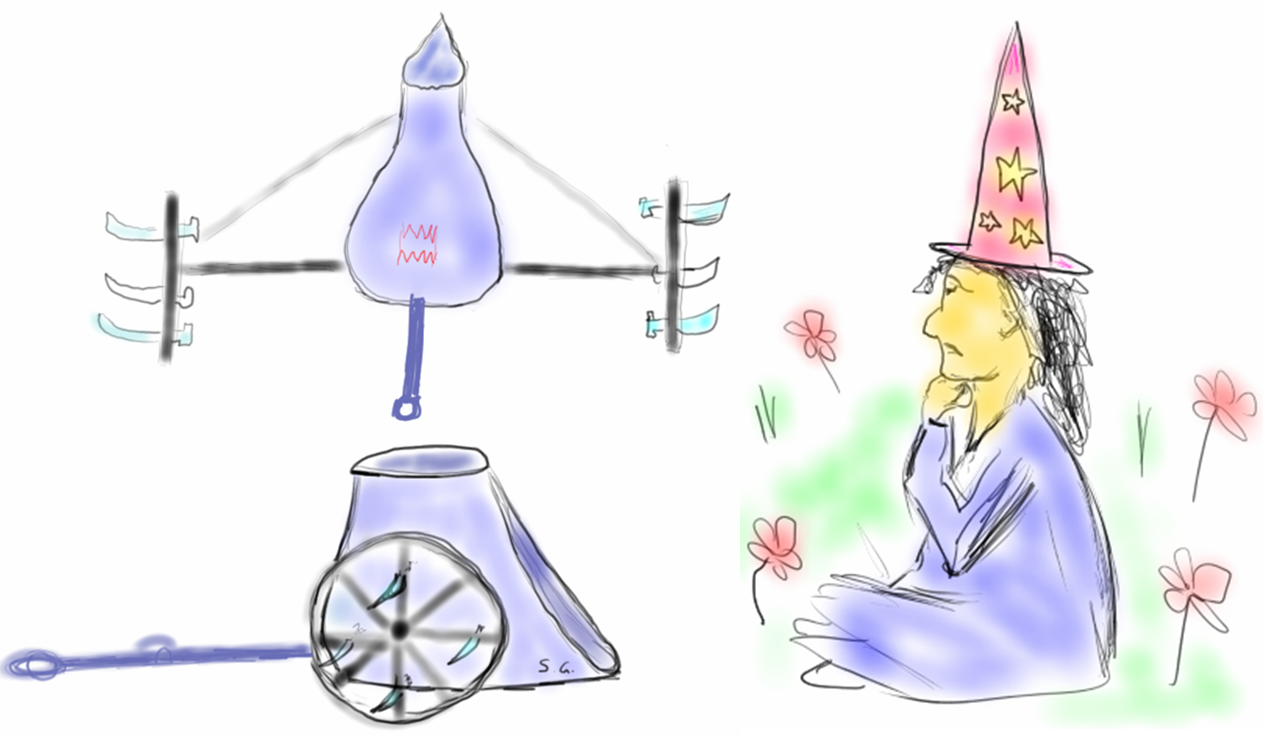
\includegraphics[scale=0.5]{6_chemestryWitch.png}
\end{center} \end{figure}
\leavevmode\makebox(0,0){\put(175,357){
\includegraphics[height=3cm]{6_cloudToTheLeft.png}}}
\leavevmode\makebox(0,0){\put(183,415){\fontfamily{comic}{\selectfont{\bf{\scriptsize {This should}}}}}}
\leavevmode\makebox(0,0){\put(190,400){\fontfamily{comic}{\selectfont{\bf{\scriptsize {do it...}}}}}}
%footer
\leavevmode\makebox(0,0){\put(-20,7){\tiny{\textcolor{gray}{Slide idea from David Hill}}}}
\leavevmode\makebox(0,0){\put(255,7){\tiny{\textcolor{gray}{Saul Greenberg}}}}
\end{frame}



%--------------------------------------
% Iuga Alexandru
% 7
% 7_tractor.png
% 7_nature.png
\begin{frame}
    \textcolor{Blue}{\textbf{\Large{Tractors}}}
    \textcolor{red}{\rule{10cm}{1mm}}

\vspace{5mm}

\LARGE\hspace{-0.6cm} \textcolor{black}{\vspace{4cm}Early design\newline}
\leavevmode\makebox(0,0){\put(102,255){\fontfamily{comic}{\selectfont{\bf \scriptsize{{high center}}}}}}
\leavevmode\makebox(0,0){\put(97,238){\fontfamily{comic}{\selectfont{\bf \scriptsize{{of gravity }}}}}}
\leavevmode\makebox(0,0){\put(95,120){\fontfamily{comic}{\selectfont{\bf \scriptsize{{narrow front}}}}}}
\leavevmode\makebox(0,0){\put(90,105){\fontfamily{comic}{\selectfont{\bf \scriptsize{{wheel base}}}}}}
\leavevmode\makebox(0,0){\put(120,170){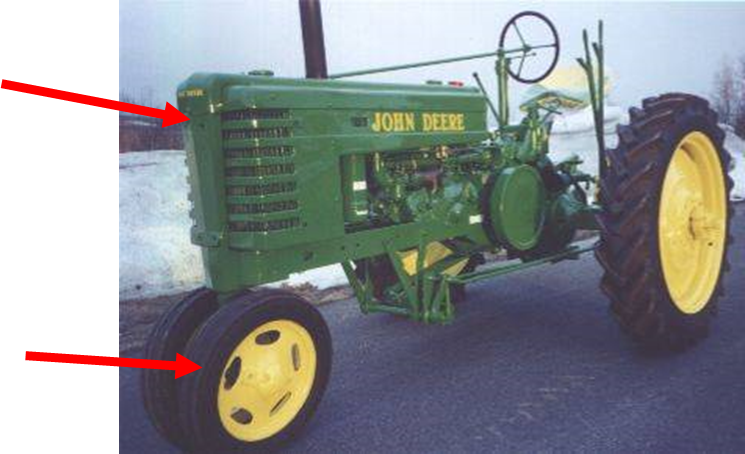
\includegraphics[scale=0.5]{7_tractor.png}}}
\leavevmode\makebox(0,0){\put(97,-150){\vspace{-2cm}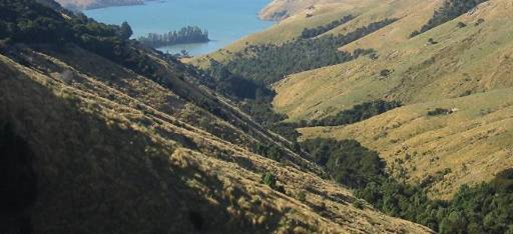
\includegraphics[scale=0.515]{7_nature.png}}}
\large \hspace{-1.4cm}\textcolor{black}{Terrain}
\begin{itemize}
  	\item[\textcolor{black}{--}] {\normalsize unsurfaced and rough}
    \item[\textcolor{black}{--}] {\normalsize hilly}
\end{itemize}
\large \textcolor{black}{Farmer}
  \begin{itemize}
  	\item[\textcolor{black}{--}] {\normalsize works long hours}
    \item[\textcolor{black}{--}] {\normalsize works quickly}
  \end{itemize}
%footer
\leavevmode\makebox(0,0){\put(-20,7){\tiny{\textcolor{gray}{Images from www.co.lawrence.tn.us and www.uni-magdeburg.de}}}}
\leavevmode\makebox(0,0){\put(275,7){\tiny{\textcolor{gray}{Saul Greenberg}}}}
\end{frame}



%------------------------------------------------
% Ivanoiu Ovidiu-Cristian
% 8
% 8_tractors.png
% 8_result.png
\begin{frame}
    \textcolor{Blue}{\textbf{\Large{Tractors}}}
    \textcolor{red}{\rule{10cm}{1mm}}

\vspace{5mm}

  {\large \textcolor{black}{}Result}
  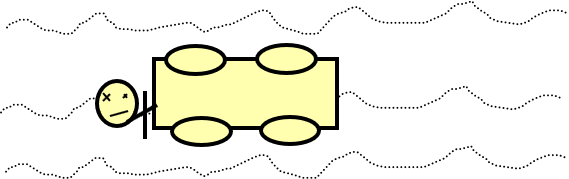
\includegraphics[scale=0.4]{8_result.png}
  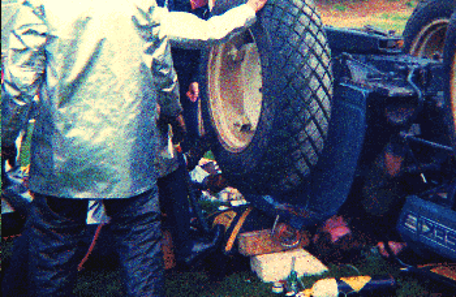
\includegraphics[scale=0.5]{8_tractors.png}
  \newline
  {\large Quotes from National AG Safety Database}
  {\begin{itemize}
  	\item[\textcolor{black}{--}] {\normalsize \textbf{older} tractors have narrow front ends that are easily upset}
    \item[\textcolor{black}{--}] {\normalsize tractor upsets cause more fatalities than other farm accidents}
    \item[\textcolor{black}{--}] {\normalsize injuries often include a broken or crushed pelvis}
  \end{itemize}}

%footer
\leavevmode\makebox(0,0){\put(-20,7){\tiny{\textcolor{gray}{Accident image from www.osh.dol.govt.nz}}}}
\leavevmode\makebox(0,0){\put(275,7){\tiny{\textcolor{gray}{Saul Greenberg}}}}
\end{frame}



%Mitaru Vlad
%slide 41
%41_tractor1.png
%41_tractor2.png
\begin{frame}
    \textcolor{Blue}{\textbf{\Large{Tractors}}}
    \textcolor{red}{\rule{10cm}{1mm}}

    \textbf{Original design}
    
\vspace{1cm}    
    
    \textbf{Terrain} 
    \begin{itemize}
      \item[\textcolor{black}{--}] un-surfaced
      \item[\textcolor{black}{--}] rough
      \item[\textcolor{black}{--}] hilly
      
      
    \end{itemize}
    \bigskip
    
\begin{picture}(0,0)
\put(110,30){\hbox{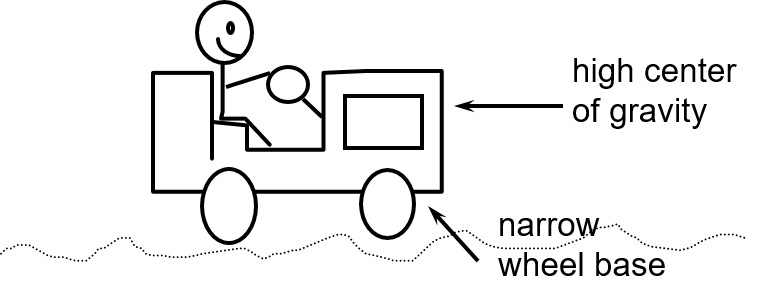
\includegraphics[scale=0.5]{41_tractor1.png}}}
\end{picture}

\begin{picture}(0,0)
\put(107,-20){\hbox{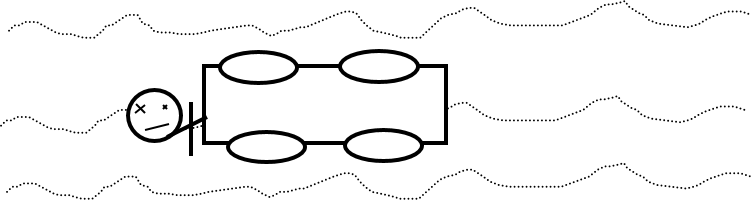
\includegraphics[scale=0.5]{41_tractor2.png}}}
\end{picture}
\bigskip
\bigskip
\bigskip
   \textbf{Result} \par
   \textbf{Used to be called driver's error}
\end{frame}



% Ivanoiu Ovidiu-Cristian
% 9
% 9_tractor.png
\begin{frame}
    \textcolor{Blue}{\textbf{\Large{Tractors}}}
    \textcolor{red}{\rule{10cm}{1mm}}

\vspace{5mm}

    {\textcolor{black}{}But:}
    {\begin{itemize}
    \item [\textcolor{black}{--}] {\normalsize \textbf{accidents less frequent as modern designs have}: }
      {\begin{itemize}
      \item[\textcolor{black}{\textbullet}] {\normalsize roll cage}
      \item[\textcolor{black}{\textbullet}] {\normalsize low center of gravity}
      \item[\textcolor{black}{\textbullet}] {\normalsize wider wheel bases}
      \end{itemize}}
    \end{itemize}}

	\begin{figure}
    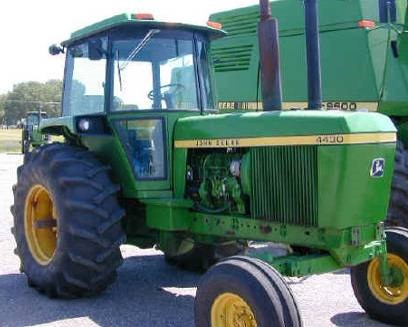
\includegraphics[scale=0.5]{9_tractor.jpg}
   	\end{figure}

\end{frame}



%------------------------------------------------
% Ivanoiu Ovidiu-Cristian
% 10
\begin{frame}
    \textcolor{Blue}{\textbf{\Large{So what does this teach us?}}}
    \textcolor{red}{\rule{10cm}{1mm}}

\vspace{5mm}

    {\large \textcolor{black}{}Lesson 1}
    {\begin{itemize}
      \item[\textcolor{black}{--}] {\normalsize many failures of human-machine system result from designs that don’t recognize peoples’ capabilities and fallibilities}
      \item[\textcolor{black}{--}] {\normalsize this leads to apparent machine misuse and human error}
      \newline
    \end{itemize}}
    
    {\large \textcolor{black}{}Lesson 2}
    {\begin{itemize}
      \item[\textcolor{black}{--}] {\normalsize good design always accounts for human capabilities}
      \newline
    \end{itemize}}
    
    {\large \textcolor{black}{}Lesson 3}
    {\begin{itemize}
      \item[\textcolor{black}{--}] {\normalsize look for examples of 'human error'}
      \item[\textcolor{black}{--}] {\normalsize critique them for possible 'design error'}
      \item[\textcolor{black}{--}] {\normalsize propose designs that limit / remove these errors}
      \newline
    \end{itemize}}
\end{frame}



%------------------------------------------------
% Ivanoiu Ovidiu-Cristian
% 11
% 11_human.png
% 11_microwave.png
% 11_watch.png
\begin{frame}
    \textcolor{Blue}{\textbf{\Large{Psychopathology of everyday things}}}
    \textcolor{red}{\rule{10cm}{1mm}}

\vspace{5mm}

    \begin{picture}(0,0)
    \put(240,-20){\hbox{
\includegraphics[scale=0.3]{11_human.png}}}
    \end{picture}
    \begin{picture}(0,0)
    \put(260,0){\hbox{
\includegraphics[scale=0.3]{11_microwave.png}}}
    \end{picture}
	\begin{picture}(0,0)
    \put(250,-170){\hbox{
\includegraphics[scale=0.4]{11_watch.png}}}
    \end{picture}

    {\large \textbf{Typical frustrations}}
    \begin{itemize}
	\item[\textcolor{black}{--}] {\normalsize The engineer who founded DEC confessed at the annual meeting that he can’t figure out how to heat a cup of coffee in the company’s microwave oven}
    \bigskip
    \item[\textcolor{black}{--}] {\normalsize How many of you can program or use all aspects of your}
    {\begin{itemize}
      \item[\textcolor{black}{\textbullet}] {\normalsize digital watch?}
      \item[\textcolor{black}{\textbullet}] {\normalsize VCR?}
      \item[\textcolor{black}{\textbullet}] {\normalsize sewing machine?}
      \item[\textcolor{black}{\textbullet}] {\normalsize washer and dryer?}
      \item[\textcolor{black}{\textbullet}] {\normalsize stereo system?}
      \item[\textcolor{black}{\textbullet}] {\normalsize cell phones?}
      \end{itemize}}
    \end{itemize}
    
%footer
    \leavevmode\makebox(0,0){\put(-15,-50){\tiny{\textcolor{gray}{Slide idea from Donald Norman}}}}
\end{frame}



%------------------------------------------------
% Ivanoiu Ovidiu-Cristian
% 12
% 12_manga.png

\begin{frame}
    \begin{picture}(0,0)
    \put(40,-167){\hbox{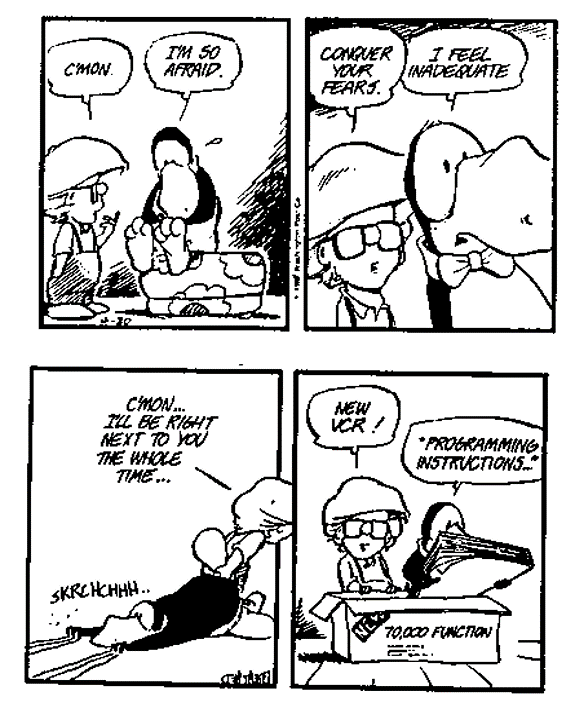
\includegraphics[scale=0.52]{12_manga.png}}}
    \end{picture}
\end{frame}



%------------------------------------------------
% Ivanoiu Ovidiu-Cristian
% 13
% 13_remote.png
\begin{frame}
    \textcolor{Blue}{\textbf{\Large{Remote Controls}}}
    \textcolor{red}{\rule{10cm}{1mm}}

    {\large \textcolor{black}{}The phone rings…}
    {\begin{itemize}
      \item[\textcolor{black}{--}] {\normalsize hit pause}
    \end{itemize}}
    
    \begin{figure}
   	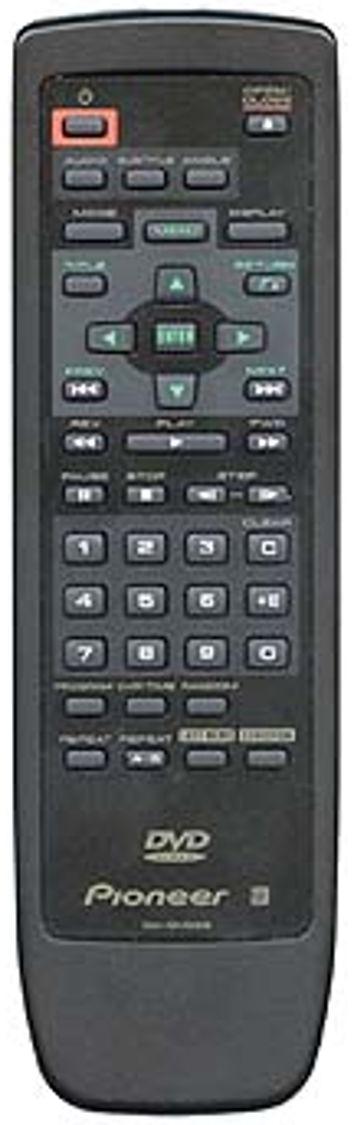
\includegraphics[scale=0.3]{13_remote.png}
    \end{figure}

	{\normalsize Pioneer DVD Remote}

\end{frame}



%------------------------------------------------
% Ivanoiu Ovidiu-Cristian
% 14
% 14_remote.png

\begin{frame}
    \textcolor{Blue}{\textbf{\Large{Remote Controls}}}
    \textcolor{red}{\rule{10cm}{1mm}}
    
    \begin{picture}(0,0)
    \put(230,-160){\hbox{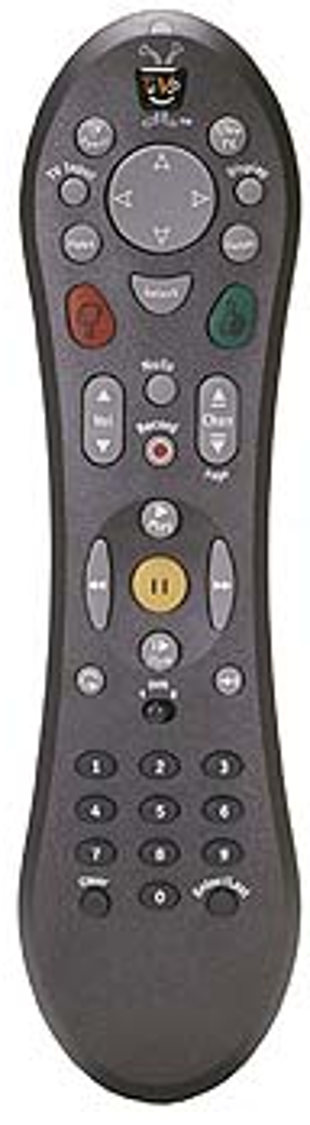
\includegraphics[scale=0.35]{14_remote.png}} \tiny {TiVo DVR}}
    \end{picture}

	{\large \textcolor{black}{}The phone rings ...}
    {\begin{itemize}
      \item[\textcolor{black}{--}] {\normalsize hit pause}
      \newline
    \end{itemize}}
    
    {\large \textcolor{black}{}Why is it easier?}
    {\begin{itemize}
      \item[\textcolor{black}{--}] {\normalsize big button easier to hit (Fitt’s Law)}
      \item[\textcolor{black}{--}] {\normalsize visually distinctive (color)}
      \item[\textcolor{black}{--}] {\normalsize reasonably different from other buttons}
      \item[\textcolor{black}{--}] {\normalsize shape and central position means its easy \newline to find by feel in zero light conditions}
      \newline
    \end{itemize}}
    
    {\large \textcolor{black}{}TiVo designed for usability}
    {\begin{itemize}
      \item[\textcolor{black}{--}] {\normalsize part of early product development}
    \end{itemize}}

%footer
    \leavevmode\makebox(0,0){\put(-15,-40){\tiny{\textcolor{gray}{Slide idea from Jacob Nielsen Alertbox March 15, 2004}}}}
\end{frame}



%------------------------------------------------
% Lica Alexandru
% 15
% 15_controllers.jpg
\begin{frame}
    \textcolor{Blue}{\textbf{\Large{Remote Controls}}}
    \textcolor{red}{\rule{10cm}{1mm}}

{\large But of course I'll just learn it quickly...}
\newline
\begin{center}
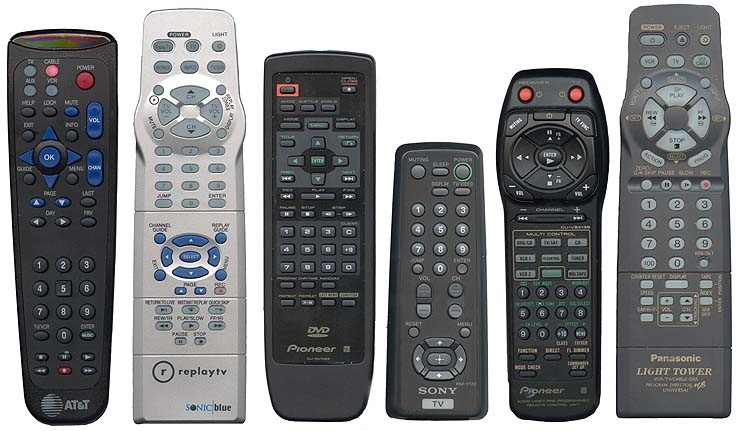
\includegraphics[scale=0.4]{15_controllers.jpg}
\end{center}
cable box \ {\tiny digital video recorder} \ DVD  \quad  television \quad {\tiny audio amplifier} \quad VCR
\newline
six remote controls required to operate a modest home theater

%footer
    \leavevmode\makebox(0,0){\put(-15,0){\tiny{\textcolor{gray}{Slide idea from Jacob Nielsen Alertbox March 15, 2004}}}}
\end{frame}



%------------------------------------------------
% Lica Alexandru
% 16
% 16_slide_projector.png
\begin{frame}
    \textcolor{Blue}{\textbf{\Large{Other pathological examples}}}
    \textcolor{red}{\rule{10cm}{1mm}}

{\large Remote control Leitz slide projector}
\newline
\begin{itemize}
	\item[\textcolor{black}{--}] {\normalsize How do you forward/reverse?}
\end{itemize}
\begin{center}
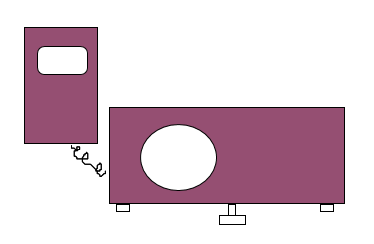
\includegraphics[scale=0.5]{16_slide_projector.png}
\end{center}

{\large Instruction manual:}
\begin{itemize}
	\item[\textcolor{black}{--}] {\normalsize \textit{short press:} \qquad slide change forward}
	\item[\textcolor{black}{--}] {\normalsize \textit{long press:} \qquad \ slide change backward}
\end{itemize}
\end{frame}



%Mitaru Vlad
%slide 40
%40_controlroom.png
\begin{frame}
    \textcolor{Blue}{\textbf{\Large{Other pathological examples}}}
    \textcolor{red}{\rule{10cm}{1mm}}

    \textbf{Amphitheater Louis-Laird in Sorbonne} \par
    \bigskip
    \begin{itemize}
      \item[\textcolor{black}{--}] beautiful room with murals on ceiling
       \begin{itemize}
        \item[\textcolor{black}{•}] but murals are right side up only for lecturer!
        \end{itemize}
        \bigskip
    \item[\textcolor{black}{--}] electric projection screen
       \begin{itemize}
        \item[\textcolor{black}{•}] controls in other room out of sight of screen!
        \end{itemize}
     
\begin{center}
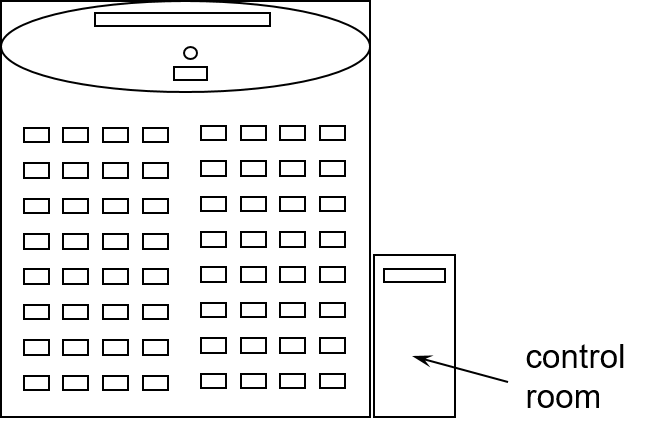
\includegraphics[scale=0.5]{40_controlroom.png} 
\end{center}
    \end{itemize}
    
%footer
    \leavevmode\makebox(0,0){\put(-15,0){\tiny{\textcolor{gray}{Slide idea from Donald Norman}}}}
\end{frame}



%------------------------------------------------
% Lica Alexandru
% 17
% 17_telephone.png
\begin{frame}
	\textcolor{Blue}{\textbf{\Large{Other pathological examples}}}
    \textcolor{red}{\rule{10cm}{1mm}}

\begin{picture}(0,0)
\put(220,-60){\hbox{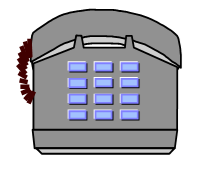
\includegraphics[scale=0.5]{17_telephone.png}}}
\end{picture}


{\large Modern telephone systems}
\begin{itemize}
	\item[\textcolor{black}{--}] {\normalsize standard number pad}
	\item[\textcolor{black}{--}] {\normalsize two additional buttons  \** and \# }
\end{itemize}

\bigskip

{\large Problem}
\begin{itemize}
	\item[\textcolor{black}{--}] {\normalsize many hidden functions}
	\item[\textcolor{black}{--}] {\normalsize operations and outcome completely invisible }
		\setbeamertemplate{itemize items}[circle]
  		\begin{itemize}
      		\item[\textcolor{black}{\textbullet}]  {\small *72+number = call forward}
      		\begin{itemize}
      		\item[\textcolor{black}{--}]  {\small can I remember that combination?}
      		\item[\textcolor{black}{--}]  {\small if I enter it, how do i know it caught?}
      		\item[\textcolor{black}{--}]  {\small how can I remember if my phone is still forwarded?}
  		\end{itemize}
  		\end{itemize}
  		\setbeamertemplate{itemize items}[circle]
  		\begin{itemize}
      		\item[\textcolor{black}{\textbullet}]  {\small Ok, I'll read the manual}
      		\begin{itemize}
      		\item[\textcolor{black}{--}]  {\small but what does call park mean? what's a link?}
      		\item[\textcolor{black}{--}]  {\small where is that manual anyway?}
  			\end{itemize}
  		\end{itemize}
  		
\end{itemize}
\end{frame}



%------------------------------------------------
% Lica Alexandru
% 18
% 18_fax.png
% 18_clock.png
\begin{frame}
    \textcolor{Blue}{\textbf{\Large{Other pathological examples}}}
    \textcolor{red}{\rule{10cm}{1mm}}
    
\begin{picture}(0,0)
\put(210,-40){\hbox{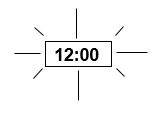
\includegraphics[scale=0.6]{18_clock.png}}}
\end{picture}

{\large VCR's, camcorders, fax machines, ...}
\begin{itemize}
	\item[\textcolor{black}{--}]  {\normalsize most people learn only basic functions}
	\item[\textcolor{black}{--}]  {\normalsize most functionality goes untouched}
\end{itemize}

\begin{center}
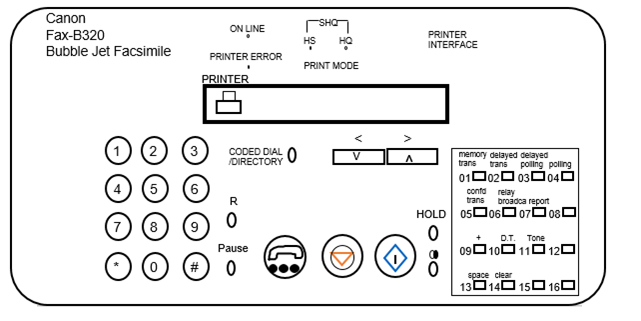
\includegraphics[scale=0.5]{18_fax.png}
\end{center}

\end{frame}



%------------------------------------------------
% Lica Alexandru
% 19
% 19_airplanes.png
\begin{frame}
    \textcolor{Blue}{\textbf{\Large{Other pathological examples}}}
    \textcolor{red}{\rule{10cm}{1mm}}

\begin{picture}(0,0)
\put(230,-20){\hbox{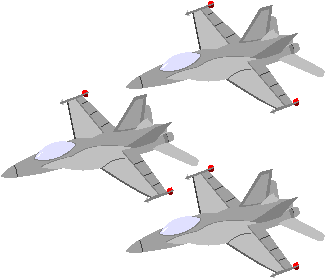
\includegraphics[scale=0.5]{19_airplanes.png}}}
\end{picture}

{\large World War II}
\begin{itemize}
	\item[\textcolor{black}{--}] {\normalsize complex machines (airplanes, submarines...)}
		\setbeamertemplate{itemize items}[circle]
  		\begin{itemize}
      		\item[\textcolor{black}{\textbullet}]  {\small taxed people's sensorimotor abilities to control them}
      		\item[\textcolor{black}{\textbullet}]  {\small frequent (often fatal) errors occured even after high 				training}
  		\end{itemize}

		\smallskip  		
  		
  	\item[\textcolor{black}{--}] {\normalsize example airplane errors: }
  		\setbeamertemplate{itemize items}[circle]
  		\begin{itemize}
      		\item[\textcolor{black}{\textbullet}]  {\small if booster pump fails turn on fuel valve within 3 					seconds}
      			\begin{itemize}
      				\item[\textcolor{black}{--}]  {\small test shows it took ~five seconds to 								actually do it}
  				\end{itemize}
  				
			\smallskip    				
  				
  			\item[\textcolor{black}{\textbullet}]  {\small Spitfire: narrow wheel base}
      			\begin{itemize}
      				\item[\textcolor{black}{--}]  {\small easy to do violent ground loops which 							breaks undercarriage}
  				\end{itemize}
  				
			\smallskip    				
  				
  			\item[\textcolor{black}{\textbullet}]  {\small Altimeter gauges difficult to read}
      			\begin{itemize}
      				\item[\textcolor{black}{--}]  {\small caused crashes when pilots believe they are 					at a certain altitude}
  				\end{itemize}
  		\end{itemize}
  		
\end{itemize}

{\large Result}
\begin{itemize}
	\item[\textcolor{black}{--}] {\normalsize human factors became critically important}
\end{itemize}

%footer
    \leavevmode\makebox(0,0){\put(-15,-10){\tiny{\textcolor{gray}{Slide ideas from David Hill}}}}
\end{frame}



%------------------------------------------------
% Lica Alexandru
% 20
% 16_slide_projector.png
\begin{frame}
    \textcolor{Blue}{\textbf{\Large{Other pathological examples}}}
    \textcolor{red}{\rule{10cm}{1mm}}

\begin{minipage}[t]{0.48\linewidth}
{\large What's the altitude?}

\begin{center}
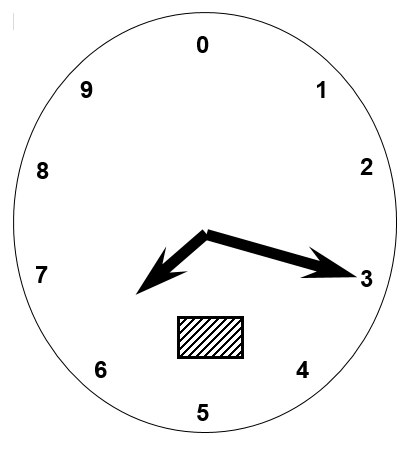
\includegraphics[scale=0.5]{20_clock.png}
\end{center}

\end{minipage}
\hfill
\begin{minipage}[t]{0.48\linewidth}
\begin{itemize}
	\item[--]  {\normalsize Early days (< 1000'):}
	\setbeamertemplate{itemize items}[circle]
  		\begin{itemize}
      		\item[\textcolor{black}{\textbullet}]  {\small only one needle needed}
  		\end{itemize}

	\item[--]  {\normalsize As ceilings increased over 1000’}
	\setbeamertemplate{itemize items}[circle]
  		\begin{itemize}
      		\item[\textcolor{black}{\textbullet}]  {\small small needle added}
  		\end{itemize}
	
	\item[--]  {\normalsize As they increased beyond 10,000’}
	\setbeamertemplate{itemize items}[circle]
  		\begin{itemize}
      		\item[\textcolor{black}{\textbullet}]  {\small box indicated 10,000' increment through color change}
      		\smallskip
      		\item[] \begin{tikzpicture}
      				\draw (0,0) rectangle (0.8,0.4);
					\end{tikzpicture}
					{\small < 10,000'}
			\smallskip
      		\item[] 
\begin{tikzpicture}
					\draw[pattern=north east lines, pattern color=black] (0,0) 							rectangle (0.8,0.4);
					\end{tikzpicture}
					{\small > 10,000'}
  		\end{itemize}	
	
\end{itemize}
\end{minipage}

%footer
    \leavevmode\makebox(0,0){\put(-15,-10){\tiny{\textcolor{gray}{Slide ideas from David Hill}}}}
\end{frame}



%------------------------------------------------
% Lica Alexandru
% 21
% 21_altimeter.png
\begin{frame}
    \textcolor{Blue}{\textbf{\Large{Other pathological examples}}}
    \textcolor{red}{\rule{10cm}{1mm}}
    
\begin{minipage}[t]{0.28\linewidth}
{\large Tape altimeter}

\begin{center}
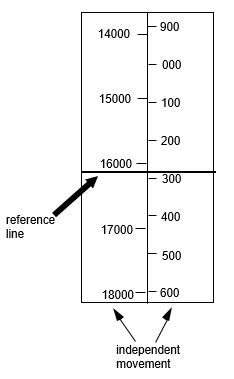
\includegraphics[scale=0.5]{21_altimeter.png}
\end{center}

\end{minipage}
\hfill
\begin{minipage}[t]{0.65\linewidth}
	\begin{itemize}
		\setbeamertemplate{itemize items}[circle]
		\item[\textcolor{black}{\textbullet}]  {\normalsize Human factors test showed:}
		\begin{itemize}
			\item[\textcolor{black}{\textbullet}]  {\small eliminate reading errors}
			\item[\textcolor{black}{\textbullet}]  {\small was faster to read}
		\end{itemize}
		\bigskip
		\bigskip
		\bigskip
		\bigskip
		\bigskip
		\bigskip
		\bigskip
		\bigskip
		\item[\textcolor{black}{\textbullet}]  {\normalsize But not in standard use! Why?}
	\end{itemize}
\end{minipage}

%footer
    \leavevmode\makebox(0,0){\put(-15,-10){\tiny{\textcolor{gray}{Slide ideas from David Hill}}}}
\end{frame}



% Lica Ion Alexandru
% 22
% 22_plane.png
% 22_land.png
\begin{frame}
    \textcolor{Blue}{\textbf{\Large{Other pathological examples}}}
    \textcolor{red}{\rule{10cm}{1mm}}
    
\textbf{Harvard Airplane (World War II)}

\begin{picture}(0,0)
\put(260,-160){\hbox{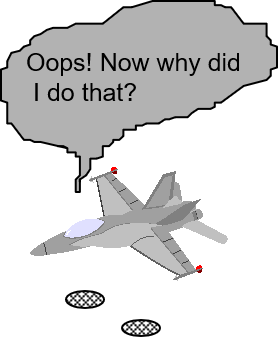
\includegraphics[scale=0.5]{22_plane.png}}}
\end{picture}

{\Large Undercarriage crashes}
\begin{itemize}
  \item[\textcolor{black}{--}] {\normalsize pilots landed without dropping undercarriage!}
  \item[\textcolor{black}{--}] {\normalsize undercarriage warning horn}

  \begin{itemize}
      \item[\textcolor{black}{\textbullet}]  {\small sounds if wheels up and power low (landing condition)}
  \end{itemize}
\end{itemize}
\bigskip
{\Large Stalls}
\begin{itemize}
  \item[\textcolor{black}{--}] {\normalsize plane airspeed drops too low to maintain lift}
  \item[\textcolor{black}{--}] {\normalsize if occurs just before landing, will crash}
  \setbeamertemplate{itemize items}[circle]
\end{itemize}
\bigskip
{\Large Training}
\begin{itemize}
  \item[\textcolor{black}{--}] {\normalsize deliberately stall and recover}
  \item[\textcolor{black}{--}] {\normalsize but sometimes similar to landing with undercarriage up}

  \begin{itemize}
      \item[\textcolor{black}{\textbullet}]  {\small horn sounds, annoyance}
  \end{itemize}
  \item[\textcolor{black}{--}] {\normalsize installed “undercarriage horn cut-out button”}
\end{itemize}
\begin{picture}(0,0)
\put(230,15){\hbox{
\includegraphics[scale=0.5]{22_land.png}}}
\end{picture}

%footer
    \leavevmode\makebox(0,0){\put(-15,-10){\tiny{\textcolor{gray}{Slide ideas from David Hill}}}}
\end{frame}



% Lica Ion Alexandru
% 23
% 23_panel.png
\begin{frame}
    \textcolor{Blue}{\textbf{\Large{Other pathological examples}}}
    \textcolor{red}{\rule{10cm}{1mm}}
    
\textbf{Harvard Airplane (World War II)}

\begin{minipage}[t]{0.48\linewidth}

\begin{picture}(0,0)
\put(10,-121){\hbox{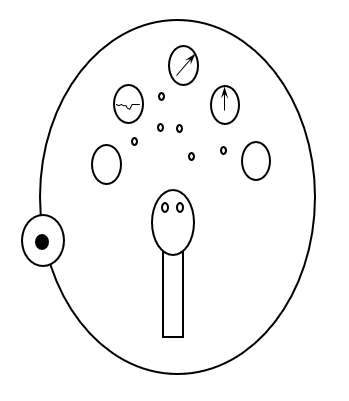
\includegraphics[scale=0.4]{23_panel.png}}}
\end{picture}

 \bigskip \bigskip \bigskip \bigskip \bigskip \bigskip

{ \ \ }
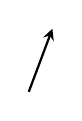
\begin{tikzpicture}[thick]
\draw [black,-stealth] (1,0) to (1.3,0.8);
\end{tikzpicture}
{\footnotesize \\ \textit{U/C horn \\
cut-out \\ 
button}}
\bigskip
\end{minipage}\hfill

{\Large Problem \#1: Conditioned response}	\\
{\large \ \ \ \ \ stall $\rightarrow$ push button; therefore stimulus nullified}

%footer
    \leavevmode\makebox(0,0){\put(-15,-10){\tiny{\textcolor{gray}{Slide ideas from David Hill}}}}
\end{frame}



% Lica Ion Alexandru
% 24
% 24_linie.png
% 24_panel_left.png
% 24_panel_right.png
\begin{frame}
    \textcolor{Blue}{\textbf{\Large{Other pathological examples}}}
    \textcolor{red}{\rule{10cm}{1mm}}
    
{\normalsize \textbf{ The Harvard Control Panel \ \ \ \ \ \ \ \ \ \ The T-33 Control Panel}}

%\begin{minipage}[t][1cm][t]{0.48\linewidth}
%\begin{center}
%{\normalsize \textbf{ The Harvard Control Panel}}
%\end{center}
%\end{minipage}\hfill
% \
%\begin{minipage}[t][1cm][t]{0.48\linewidth}
%\begin{center}
%{\normalsize \textbf{The T-33 Control Panel}}
%\end{center}
%\end{minipage}

\begin{picture}(0,0)
\put(155,-170){\hbox{
\includegraphics[scale=0.5]{24_line.png}}}
\end{picture}

\begin{minipage}{0.48\linewidth}
\begin{picture}(0,0)
\put(10,-121){\hbox{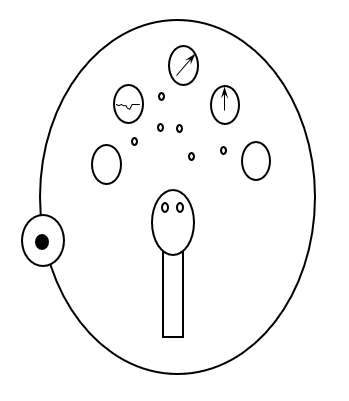
\includegraphics[scale=0.4]{24_panel_left.png}}}
\end{picture}

\bigskip \bigskip \bigskip \bigskip \bigskip \bigskip

{ \ \ }
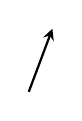
\begin{tikzpicture}[thick]
\draw [black,-stealth] (1,0) to (1.3,0.8);
\end{tikzpicture}
{\footnotesize \\ \textit{U/C horn \\cut-out \\ button}}
\bigskip
\end{minipage}\hfill
  \
\begin{minipage}{0.48\linewidth}
\begin{picture}(0,0)
\put(10,-121){\hbox{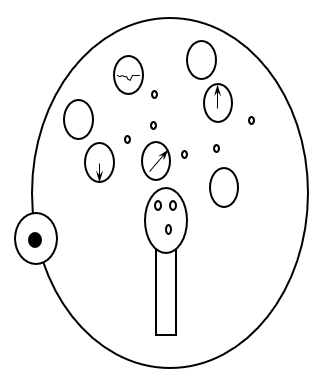
\includegraphics[scale=0.4]{24_panel_right.png}}}
\end{picture}

\bigskip \bigskip \bigskip \bigskip \bigskip \bigskip

{ \ \ }
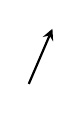
\begin{tikzpicture}[thick]
\draw [black,-stealth] (1,0) to (1.3,0.7);
\end{tikzpicture}
{\footnotesize \\ \textit{Tip-tank \\ jettison \\ button}}
\bigskip \bigskip
\end{minipage}
{\Large Problem \#2: Negative transfer}	\\
{\Large \ \ \ \ T-33’s: tip-tank jettison button in same location}

%footer
    \leavevmode\makebox(0,0){\put(-15,-10){\tiny{\textcolor{gray}{Slide ideas from David Hill}}}}
\end{frame}



% Lica Ion Alexandru
% 25
% 25_alien.png
\begin{frame}
\begin{center}
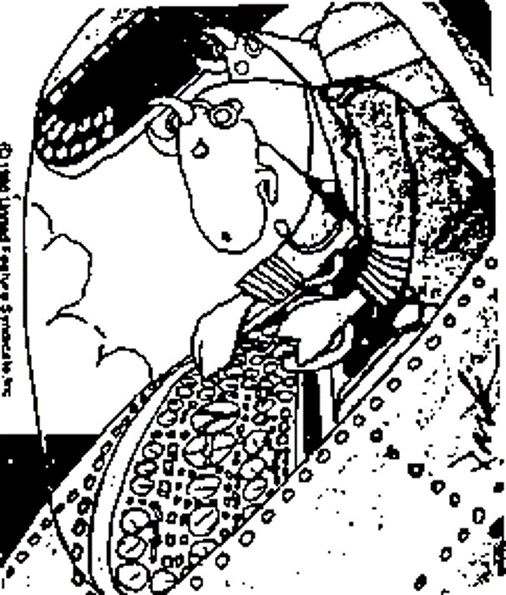
\includegraphics[scale=0.45]{25_alien.png}
\end{center}
{\Large Darn these hooves! I hit the wrong switch again!
Who designs these instrument panels, raccoons?}
\end{frame}



% Lica Ion Alexandru
% 26
% 26_road.png
\begin{frame}
    \textcolor{Blue}{\textbf{\Large{The psychopathology of computers}}}
    \textcolor{red}{\rule{10cm}{1mm}}

{\Large Britain 1976 }
\begin{itemize}
  \item[\textcolor{black}{--}] {\small Motorway communication system operated 40\% of it’s highways}
  \item[\textcolor{black}{--}] {\small police controlled it in real time to }
  \begin{itemize}
      \item[\textcolor{black}{\textbullet}]  {\small change lane signs, direction signs, speed limits, etc.}
  \end{itemize}
	\bigskip  
  \item[\textcolor{black}{--}] {\small On December 10th, police failed to change the \\ speed limit signs when fog descended }
  \begin{itemize}
      \item[\textcolor{black}{\textbullet}]  {\small 34 vehicles crashed}
      \item[\textcolor{black}{\textbullet}]  {\small 3 people killed}
      \item[\textcolor{black}{\textbullet}]  {\small 11 people injured and trapped in their vehicles}
      \item[\textcolor{black}{\textbullet}]  {\small motorway closed for 6.5 hours}
  \end{itemize}
\end{itemize}

\begin{picture}(0,0)
\put(225,-35){\hbox{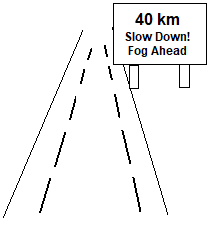
\includegraphics[scale=0.5]{26_road.png}}}
\end{picture}

%footer
    \leavevmode\makebox(0,0){\put(-15,-70){\tiny{\textcolor{gray}{Slide ideas from David Hill}}}}
\end{frame}



% Lica Ion Alexandru
% 27
% 27_notme.png
% 27_people.png
\begin{frame}
    \textcolor{Blue}{\textbf{\Large{The psychopathology of computers}}}
    \textcolor{red}{\rule{10cm}{1mm}}

{\normalsize Police (at inquest) }

\begin{itemize}
  \item[\textcolor{black}{--}] {\footnotesize "The system did not accept the instruction"}
\end{itemize}

\smallskip
{\normalsize Dept of Transport (after examining computer logs)}
\begin{itemize}
  \item[\textcolor{black}{--}] {\footnotesize “There is no evidence of technical failure”}
\end{itemize}

\smallskip
{\normalsize System designers}
\begin{itemize}
  \item[\textcolor{black}{--}] {\footnotesize after emphasizing that they have no responsibility for the system}
  \begin{itemize}
      \item[\textcolor{black}{\textbullet}]  {\scriptsize “We supplied it over 5 years ago and have never been called \\ to look at that problem”}
  \end{itemize}
\end{itemize}

\smallskip
{\normalsize The Coroner’s court}
\begin{itemize}
  \item[\textcolor{black}{--}] {\footnotesize judged it as "operator error"}
  \begin{itemize}
      \item[\textcolor{black}{\textbullet}]  {\scriptsize the police operator:\\
    “failed to follow written instructions for entering the relevant data”
}
  \end{itemize}
\end{itemize}

\bigskip
{\LARGE \textit{Where have we heard this before?}}

\begin{picture}(0,0)
\put(286,52){\hbox{
\includegraphics[scale=0.5]{27_notme.png}}}
\end{picture}
\begin{picture}(0,0)
\put(250,-9){\hbox{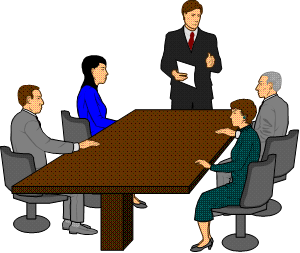
\includegraphics[scale=0.5]{27_people.png}}}
\end{picture}
\end{frame}


% Lica Ion Alexandru
% 28
\begin{frame}
    \textcolor{Blue}{\textbf{\Large{The psychopathology of computers}}}
    \textcolor{red}{\rule{10cm}{1mm}}
    
{\LARGE{{Example problems}}}

{\normalsize cryptic input codes }
\begin{itemize}
  \item[\textcolor{black}{--}] {\footnotesize XR300/1: change (X)  sign 300 on highway M5 (R) to code 1 }
  \item[\textcolor{black}{--}] {\footnotesize i.e. change particular sign to indicate fog condition}
\end{itemize}
\bigskip

{\normalsize no feedback}
\begin{itemize}
  \item[\textcolor{black}{--}] {\footnotesize operator entered command, no visible effect of system response}
\end{itemize}
\bigskip

{\normalsize cryptic error messages}
\begin{itemize}
  \item[\textcolor{black}{--}] {\footnotesize “Error code 7”}
\end{itemize}
\bigskip

{\normalsize teletype machine was old, text illegible}
\begin{itemize}
  \item[\textcolor{black}{--}] {\footnotesize people could not see what they typed or system’s reply}
\end{itemize}
\bigskip

{\normalsize operator overloaded with other chores}
\begin{itemize}
  \item[\textcolor{black}{--}] {\footnotesize also handled radio and telephone traffic}
\end{itemize}
\end{frame}



% Matei Alexandru
% slide 29
\begin{frame}
    \textcolor{Blue}{\textbf{\Large{The psychopathology of computers}}}
    \textcolor{red}{\rule{10cm}{1mm}}
    
{\LARGE{{Psychopathology of the single key press}}}

\vspace{5mm}

	\Large{from InfoWorld, Dec ’86}
    \normalsize
	\begin{itemize}
 		\item[\textcolor{black}{--}] "London-- \newline
 		\item[\textcolor{black}{}] An inexperienced computer operator pressed the wrong key on a terminal in early December, causing chaos at the London Stock Exchange. The error at [the stockbrokers office] led to systems staff working through the night in an attempt to cure the problem”
	\end{itemize}
    
    \AddToShipoutPictureFG*{
    \AtPageLowerLeft{
      \put(-3,2){
        \makebox[\paperwidth][r]{\fontsize{2pt}	{1pt}\selectfont{\color{gray}{Saul Greenberg}}}
      }
    }  
   }

\end{frame}



% Matei Alexandru
% slide 30
\begin{frame}
    \textcolor{Blue}{\textbf{\Large{The psychopathology of computers}}}
    \textcolor{red}{\rule{10cm}{1mm}}
    
{\LARGE{{Psychopathology of the single key press}}}

\vspace{5mm}

    \Large{ from \textit{Science} magazine}
    \normalsize
    \begin{itemize}
 		\item[\textcolor{black}{--}] In 1988, the Soviet Union’s Phobos 1 satellite was lost on its way to Mars, when it went into a tumble from which it never recovered. \newline
        \item[\textcolor{black}{}] “not long after the launch, a ground controller omitted a single letter in a series of digital commands sent to the spacecraft. And by malignant bad luck, that omission caused the code to be mistranslated in such a way as to trigger the [ROM] test sequence [that was intended to be used only during checkout of the spacecraft on the ground]”
	
	\end{itemize}
    
    \AddToShipoutPictureFG*{
    \AtPageLowerLeft{
      \put(-3,2){
        \makebox[\paperwidth][r]{\fontsize{2pt}	{1pt}\selectfont{\color{gray}{Saul Greenberg}}}
      }
    }  
}
\end{frame}



% Matei Alexandru
% slide 31
\begin{frame}
    \textcolor{Blue}{\textbf{\Large{The psychopathology of computers}}}
    \textcolor{red}{\rule{10cm}{1mm}}
    
{\LARGE{{The PC Cup Holder}}}

\vspace{5mm}

    \normalsize{A true (?) story from a Novell NetWire SysOp} \newline
    %am incercat doua metode de a folosi dialogue, dar imi da eroare la end frame, asa ca voi hardcoda
    %\newcommand{\dialogueline}[2]{\begin{dialogue}{#1} #2 \end{dialogue}}
    %\dialogueline{Caller}{Hello, } 
    %
    %\begin{dialogue}
    	%\speak{Caller} Hello, is this Tech Support?"
   	%\end{dialogue}
 	\scriptsize
    \begin{itemize}
    	\item[\textcolor{black}{ }] Caller: \qquad \enspace Hello, is this Tech Support?"
        \item[\textcolor{black}{ }] Tech Rep: \quad Yes, it is. How may I help you? 
        \item[\textcolor{black}{ }] Caller: \qquad \enspace The cup holder on my PC is broken and I am within my warranty \tab \qquad \enspace period. How do I go about getting that fixed? 
         \item[\textcolor{black}{ }] Tech Rep: \quad I'm sorry, but did you say a cup holder?
         \item[\textcolor{black}{ }] Caller: \qquad \enspace Yes, it's attached to the front of my computer.
        \item[\textcolor{black}{ }] Tech Rep: \quad Please excuse me if I seem a bit stumped, it's because I am. Did \tab \qquad \enspace you receive this as part of a promotional, at a trade show? How \tab \qquad \enspace did you get this cup holder? Does it have any trademark on it?
        \item[\textcolor{black}{ }] Caller: \qquad \enspace It came with my computer, I don't know anything about a \tab \qquad \enspace promotional. It just has '4X' on it. 
    \end{itemize} \par
    \   \\
    \footnotesize{At this point the Tech Rep had to mute the call, because he couldn't stand it.}\newline
  
    \footnotesize{The caller had been using the load drawer of the CD-ROMdrive as a cup holder, and snapped it off the drive.}
    
    \AddToShipoutPictureFG*{

    \AtPageLowerLeft{
      \put(-3,2){
        \makebox[\paperwidth][r]{\fontsize{2pt}	{1pt}\selectfont{\color{gray}{Saul Greenberg}}}
      }
    }  
}
    
\end{frame}



\begin{frame}
    \textcolor{Blue}{\textbf{\Large{*The psychopathology of computers}}}
    \textcolor{red}{\rule{10cm}{1mm}}
    
{\LARGE{{Reported in the Human Factors Society Bulletin, 1981}}}

\begin{itemize}
\item
the manager of a system installation for police departments reported that one day he received the call "Your terminal is dead. Come and get it."
\item
He suggested that the repair service should be contacted, but the caller insisted.
\item
The terminal had two bullet holes in it.
\item
Apparently, an officer got a "\textit{Do not understand}" message on the screen once too often.
\end{itemize}

%footer
    \leavevmode\makebox(0,0){\put(-15,-70){\tiny{\textcolor{gray}{Slide from Keith Andrews}}}}
\end{frame}



\begin{frame}
    \textcolor{Blue}{\textbf{\Large{*The psychopathology of computers}}}
    \textcolor{red}{\rule{10cm}{1mm}}
    
{\LARGE{{Iran Air 655}}}

\begin{itemize}
\item
USS Vincennes shot down an Iran Air A-300 Airbus with 290 people aboard (1988)

\item
it used the Aegis weapons system with \textbf{sophisticated software} for identifying and tracking potential targets

\item
however, the large-screen display did not show altitude information

\item
so altitude had to be read from separate consoles

\item
the Airbus which had levelled off at 12 500 feet, was taken to be an F-14 fighter descending from 9 000 feet

\item
ironically, an escort ship with older equipment was able to read the plane's altitude quite correctly, but could not intervene in time.
\end{itemize}

%footer
    \leavevmode\makebox(0,0){\put(-15,-10){\tiny{\textcolor{gray}{Slide from Keith Andrews, idea credited to L. Lee}}}}
\end{frame}



\begin{frame}
    \textcolor{Blue}{\textbf{\Large{*The psychopathology of computers}}}
    \textcolor{red}{\rule{10cm}{1mm}}
    
{\LARGE{{Beware Unix Commands}}}

\begin{itemize}
\item
intend to type: rm *\~\ to remove Emacs backup files

\item
actually type: rm * \~\ which removes everything!

\item
and there is no undo ...
\end{itemize}

%footer
    \leavevmode\makebox(0,0){\put(-15,-180){\tiny{\textcolor{gray}{Slide from Keith Andrews}}}}
\end{frame}



\begin{frame}
    \textcolor{Blue}{\textbf{\Large{*The psychopathology of computers}}}
    \textcolor{red}{\rule{10cm}{1mm}}
    
{\LARGE{{Smallest Setting is 1\%}}}

\begin{itemize}
\item
Internet Explorer 4.0 cache size could only be set in increments of 1\% of the size of the hard disk

\item
"\textit{The smallest setting is 1\%. I have a 4 Gig drive, and don't need 40 MB of cache, thank you.}" (Ross Cormier)
\end{itemize}

\begin{figure}
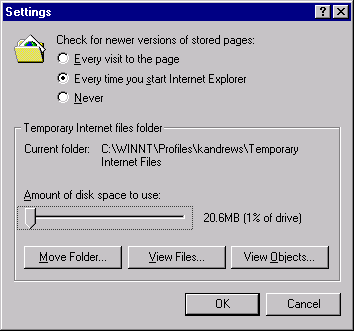
\includegraphics[scale=0.5]{ka1.png}
\end{figure}

%footer
    \leavevmode\makebox(0,0){\put(-15,-10){\tiny{\textcolor{gray}{Slide from Keith Andrews}}}}
\end{frame}



\begin{frame}
    \textcolor{Blue}{\textbf{\Large{*The psychopathology of computers}}}
    \textcolor{red}{\rule{10cm}{1mm}}
    
{\LARGE{{Horizontal Scrolling}}}

\begin{itemize}
\item
Internet Explorer 4.0 certificate authority selection panel uses horizontal scrolling

\item
humans can scan written material \textbf{faster from top to bottom} rather than left to right
\end{itemize}

\begin{figure}
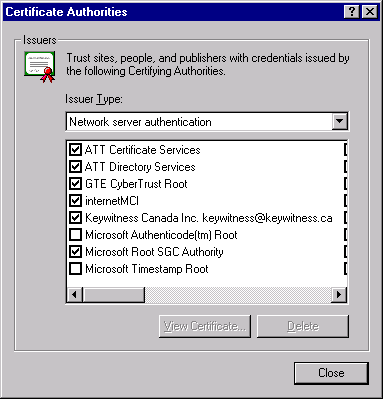
\includegraphics[scale=0.5]{ka2.png}
\end{figure}

%footer
    \leavevmode\makebox(0,0){\put(-15,-10){\tiny{\textcolor{gray}{Slide from Keith Andrews}}}}
\end{frame}



\begin{frame}
    \textcolor{Blue}{\textbf{\Large{*The psychopathology of computers}}}
    \textcolor{red}{\rule{10cm}{1mm}}
    
{\LARGE{{Two Item List Box}}}

\begin{itemize}
\item
Visual Basic 5.0 used a two item list box

\item
a drop down list or radio buttons would have been preferable
\end{itemize}

\begin{figure}
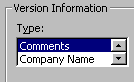
\includegraphics[scale=1]{ka3.png}
\end{figure}

%footer
    \leavevmode\makebox(0,0){\put(-15,-100){\tiny{\textcolor{gray}{Slide from Keith Andrews}}}}
\end{frame}



\begin{frame}
    \textcolor{Blue}{\textbf{\Large{*The psychopathology of computers}}}
    \textcolor{red}{\rule{10cm}{1mm}}
    
{\LARGE{{Two Thousand Item List Box}}}

\begin{itemize}
\item
do not put hundreds or thousands of items into a list box, either 

\item
"\textit{I want to fill a list box with 2000 items ... This takes incredibly long ... over 20 minutes. Any ideas?}" 

(a Visual Basic programmers forum, 1996)
\end{itemize}

\begin{figure}
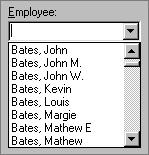
\includegraphics[scale=1]{ka4.png}
\end{figure}

%footer
    \leavevmode\makebox(0,0){\put(-15,-10){\tiny{\textcolor{gray}{Slide from Keith Andrews}}}}
\end{frame}



\begin{frame}
    \textcolor{Blue}{\textbf{\Large{*The psychopathology of computers}}}
    \textcolor{red}{\rule{10cm}{1mm}}
    
{\LARGE{{Multi-Row Property Sheets}}}

\begin{itemize}
\item
tab controls are among the best user interface elements ever devised

\item
multi-row tab controls are perhaps one of the worst interface elements ever!

\item
clicking one of the tabs other than from the bottom row, causes a major reorganisation of the complete set of tabs
\end{itemize}

\begin{figure}
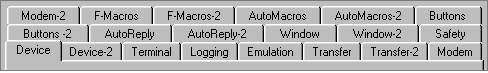
\includegraphics[scale=1]{ka5.png}
\end{figure}

%footer
    \leavevmode\makebox(0,0){\put(-15,-40){\tiny{\textcolor{gray}{Slide from Keith Andrews}}}}
\end{frame}



% Matei Alexandru
% slide 32
% 32_SourceSafe.png
% 32_Saving.png
% 32_AXE.png
% 32_ok.png
\begin{frame}
    \textcolor{Blue}{\textbf{\Large{The psychopathology of computers}}}
    \textcolor{red}{\rule{10cm}{1mm}}
    
{\LARGE{{Inane Dialog Boxes}}}

\vspace{-5mm}

%     \begin{picture}(0,0)
% 		\put(-20,0){\hbox{
\includegraphics[scale=0.5]{32_SourceSafe.png}}}
% 	\end{picture}

\begin{columns}[t]
\column{.5\textwidth}
\centering
\begin{figure}[H]
	\begin{flushleft}
	\includegraphics[width=5.2cm,height=2cm]{32_SourceSafe.png}\\
	Umm, thanks for the warning, but what should I do?
    \end{flushleft}
\end{figure}
\begin{figure}[H]
	\begin{flushleft}
	\includegraphics[width=5.7cm,height=2cm]{32_AXE.png}
    \\ Do I have any choice in this?
    \end{flushleft}
\end{figure}
\column{.5\textwidth}
\centering
\begin{figure}[H]
	\begin{flushleft}
	\includegraphics[width=5.3cm,height=2cm]{32_Saving.png}\\
	What happens when you cancel a cancelled operation?
    \end{flushleft}
\end{figure}
\begin{figure}[H]
	\begin{flushleft}
	%\advance\leftskip-1.5cm
    \ \\
	\includegraphics[width=3.3cm,height=1.5cm]{32_ok.png}
    \ \\ \vspace{5mm}  Uhhh… I give up on this one 
    \end{flushleft}
\end{figure}
\end{columns}   
\end{frame}
 
 
 
% Matei Alexandru
% slide 33
% 33_revision.png
% 33_netinfo.png
% 33_mosaix.png
\begin{frame}
    \textcolor{Blue}{\textbf{\Large{The psychopathology of computers}}}
    \textcolor{red}{\rule{10cm}{1mm}}
    
{\LARGE{{Inane Dialog Boxes}}}

\includegraphics[scale=0.5]{33_revision.png}
\vspace{5mm}
\begin{picture}(0,0)
		\put(-30,-45){\hbox{\includegraphics[scale=0.5]{33_netinfo.png}}}
\end{picture}
\includegraphics[scale=0.5]{33_mosaix.png}

\AddToShipoutPictureFG*{

    \AtPageLowerLeft{
    	\put(-190,2){
        \makebox[\paperwidth][r]{\fontsize{0.5pt}	{0.1pt}\selectfont{\color{gray}{Some of these interfaces were posted on Interface Hall of Shame
}}}
      }
      \put(-3,2){
        \makebox[\paperwidth][r]{\fontsize{2pt}	{1pt}\selectfont{\color{gray}{Saul Greenberg}}}
      }
    }  
}

\end{frame}



% Matei Alexandru
% slide 34
% 34_javascript.png
\begin{frame}
    \textcolor{Blue}{\textbf{\Large{The psychopathology of computers}}}
    \textcolor{red}{\rule{10cm}{1mm}}
    
{\LARGE{{Inane Dialog Boxes}}}
\newline

\normalsize{\textit{Midwest Microwave's} online catalog}
\includegraphics[scale=0.5]{34_javascript.png}

\AddToShipoutPictureFG*{

    \AtPageLowerLeft{
    	\put(-190,2){
        \makebox[\paperwidth][r]{\fontsize{0.5pt}	{0.1pt}\selectfont{\color{gray}{Some of these interfaces were posted on Interface Hall of Shame
}}}
      }
      \put(-3,2){
        \makebox[\paperwidth][r]{\fontsize{2pt}	{1pt}\selectfont{\color{gray}{Saul Greenberg}}}
      }
    }  
}
\end{frame}



% Matei Alexandru
% slide 35
% 35_baterry.png
% 35_optout.png
% 35_error.png
% 35_diff.png
% 35_turbo.png
\begin{frame}
    \textcolor{Blue}{\textbf{\Large{The psychopathology of computers}}}
    \textcolor{red}{\rule{10cm}{1mm}}
    
{\LARGE{{Inane Dialog Boxes}}}
\newline

\vspace{5mm}

\begin{columns}[t]

\column{.5\textwidth}
	\vspace{-1cm}
	\includegraphics[scale=0.5]{35_battery.png} 
	\vspace{2mm}
	\includegraphics[scale=0.5]{35_optout.png}
	\vspace{2mm}
	\includegraphics[scale=0.5]{35_error.png}
    \hspace{-8mm}
\column{.5\textwidth}
	\vspace{-1cm}
	\includegraphics[scale=0.5]{35_diff.png}
    %\hspace{-4mm}
	%\tiny{\textrm{\textit{ClearCase}, source-code control Rational Software}}
   	\vspace{-2mm}
    \scalebox{0.6}{\textit{ClearCase}, source-code control Rational Software}\\
    \vspace{8mm}
    \includegraphics[scale=0.5]{35_turbo.png}
\end{columns}
\end{frame}



%Mitaru Vlad
%slide 36

\begin{frame}{}

\begin{center}
\includegraphics[scale=0.5]{27_duck.png} 
\end{center}

\begin{center}
{\Large \textbf{"HIT ANY KEY TO CONTINUE"}}
\end{center}

\end{frame}



%Mitaru Vlad
%slide 37
\begin{frame}
    \textcolor{Blue}{\textbf{\Large{Why should you care?}}}
    \textcolor{red}{\rule{10cm}{1mm}}

    \textbf{Past} \par
    \begin{itemize}
      \item[\textcolor{black}{--}] manufacturers had little incentive to emphasize usability
      \item[\textcolor{black}{--}] customers have no experience until after they buy the product
      \item[\textcolor{black}{--}] early technology adaptors were ‘resilient’ 
 \begin{itemize}
        \item[\textcolor{black}{•}] willing to put up with annoyances
        
      \end{itemize}
      
      \item[\textcolor{black}{--}] consequences of bad design typically small (annoyances)
    \end{itemize}
    
    %footer
    \leavevmode\makebox(0,0){\put(-15,-150){\tiny{\textcolor{gray}{Slide idea from Jacob Nielsen Alertbox March 15, 2004}}}}
\end{frame}



%Mitaru Vlad
%slide 38
\begin{frame}
    \textcolor{Blue}{\textbf{\Large{Why should you care?}}}
    \textcolor{red}{\rule{10cm}{1mm}}
	
   \textbf{ Today: Usability sells} \par
    \begin{itemize}
      \item[\textcolor{black}{--}] product reviews emphasize usability (e.g., Consumer Reports)
      \item[\textcolor{black}{--}] customers have used related products, and can often download trial versions (including competitors)
      \item[\textcolor{black}{--}] today's users are impatient and intolerant of bad design
    \end{itemize}
    \bigskip
    \textbf{Consequences of bad design now large}
    \begin{itemize}
      \item[\textcolor{black}{--}] costly errors in serious systems (e.g. financial institutes)

      \item[\textcolor{black}{--}] widespread effects (e.g. incorrect billing, failures)

    
      \item[\textcolor{black}{--}] life-critical systems (e.g. medical, air traffic control)
		\item[\textcolor{black}{--}] safety (e.g. in-car navigation systems) 
    \end{itemize}
\end{frame}



%Mitaru Vlad
%slide 39
\begin{frame}
    \textcolor{Blue}{\textbf{\Large{Why should you care?}}}
    \textcolor{red}{\rule{10cm}{1mm}}
	
   \textbf{Professionalism} \par
    \begin{itemize}
      \item[\textcolor{black}{--}] software engineers are designers 

      \item[\textcolor{black}{--}] we are ultimately responsible for the products we build

      \item[\textcolor{black}{--}] a history of ‘hack’ designs does not excuse our responsibilities

    \end{itemize}
    \bigskip
    \textbf{Compared to civil engineers}

    \begin{itemize}
      \item[\textcolor{black}{--}] What would happen to an engineer who built a bridge where people fell off of it into the river (because the guard rails were too low), and where accidents were high (because the bridge was too narrow)? 

      \item[\textcolor{black}{--}] We would call this incompetence. 

      \item[\textcolor{black}{--}] \textbf{The same standard should apply to software engineers.}

    \end{itemize}
    
\end{frame}



{\setbeamercolor{background canvas}{bg=background}
\setbeamercolor{normal text}{fg=Blue}
\usebeamercolor[fg]{normal text}
\begin{frame}
	\vspace{8mm}
	\textcolor{Blue}{\textbf{\Large{*Bibliography}}}
    \textcolor{red}{\rule{10cm}{1mm}}

        \begin{itemize}
        	\item[{$\bullet$}] Saul Greenberg, \textbf{Designing and building visual interfaces. Pathological designs}, University of Calgary, Canada

        	\url{http://pages.cpsc.ucalgary.ca/~saul/481/}
        	\newline
        	 
        	\item[{$\bullet$}] Keith Andrews, \textbf{Human Computer Interaction, Chapter 2. The Psychology of Usable Things}, TU Graz, Austria

        	\url{https://courses.isds.tugraz.at/hci/hci.pdf}                			\newline
     	\end{itemize}
\end{frame}



\end{document}